\chapter{Komplexe Zahlen}

\section{Einf\"{u}hrung und Definition}
Die Gleichung $x^2 = -1$ hat in den reellen Zahlen keine L\"{o}sung.  Wir wollen uns \"{u}berlegen,
dass es m\"{o}glich ist, die Menge der reellen Zahlen so zu erweitern, dass die
Gleichung $x^2 = -1$ doch eine L\"{o}sung hat.  Bezeichnen wir diese L\"{o}sung mit $i$, so muss
f\"{u}r dieses $i$ also
\\[0.2cm]
\hspace*{1.3cm}
$i \cdot i = -1$
\\[0.2cm]
gelten.  Wir definieren dazu die Menge $\mathbb{C}$ der \emph{komplexen Zahlen} als Menge
von Paaren
\\[0.2cm]
\hspace*{1.3cm}
\colorbox{red}{\framebox{\colorbox{blue}{\framebox{\colorbox{yellow}{
$\mathbb{C} := \{ \pair(x,y) \mid x \in \mathbb{R} \wedge y \in \mathbb{R} \}$,}}}}}
\\[0.2cm]
wobei wir das Paar $\pair(x,y)$ als die Zahl $x + i \cdot y$ interpretieren:
\\[0.2cm]
\hspace*{1.3cm}
$\pair(x,y) \;\widehat{=}\; x + i \cdot y$.
\\[0.2cm]
Unser Ziel ist es, auf der Menge $\mathbb{C}$ Operationen $+$ und $\cdot$ so einzuf\"{u}hren, dass
die Struktur
\\[0.2cm]
\hspace*{1.3cm}
$\langle \mathbb{C}, \pair(0,0), \pair(1,0), +, \cdot \rangle$
\\[0.2cm]
mit diesen Operationen ein K\"{o}rper wird und dass, wenn wir 
\\[0.2cm]
\hspace*{1.3cm}
\colorbox{red}{\framebox{\colorbox{blue}{\framebox{\colorbox{yellow}{$i := \langle 0, 1 \rangle$}}}}} 
\quad definieren, die Gleichung \quad
\colorbox{red}{\framebox{\colorbox{blue}{\framebox{\colorbox{yellow}{$i \cdot i = -1$}}}}}
\\[0.2cm]
erf\"{u}llt ist.  
Zun\"{a}chst definieren wir auf den komplexen Zahlen eine Addition, indem wir 
\\[0.2cm]
\hspace*{1.3cm}
$\pair(x_1,y_1) + \pair(x_2, y_2) := \pair(x_1 + x_2, y_1 + y_2)$
\\[0.2cm]
definieren, denn wir haben
\\[0.2cm]
\hspace*{1.3cm}
$
\begin{array}[t]{lcl}
\pair(x_1,y_1) + \pair(x_2, y_2) & \widehat{=} & x_1 + i \cdot y_1 + x_2 + i \cdot y_2 \\[0.2cm]
                                & =           & (x_1 + x_2) + i \cdot (y_1 + y_2)     \\[0.2cm]
                                & \widehat{=} & \pair(x_1 + x_2, y_1 + y_2)
\end{array}
$
\\[0.2cm]
Es ist leicht nachzurechnen, dass f\"{u}r die so definierte Addition von Paaren
sowohl das Assoziativ-Gesetz als auch das Kommutativ-Gesetz gilt und dass weiterhin das
Paar $\pair(0,0)$ ein neutrales Element 
dieser Addition ist.  Au\3erdem ist klar, dass mit dieser Definition das Paar
$\pair(-x,-y)$ bez\"{u}glich der Addition ein inverses Element ist.  Wir definieren daher
\\[0.2cm]
\hspace*{1.3cm}
$-\pair(x,y) := \pair(-x,-y)$.
\\[0.2cm]
Damit ist die Struktur
\\[0.2cm]
\hspace*{1.3cm}
$\langle \mathbb{C}, \pair(0,0), + \rangle$
\\[0.2cm]
eine kommutative Gruppe.
Als n\"{a}chstes wollen wir f\"{u}r die komplexe Zahlen eine Multiplikation einf\"{u}hren.   Das Ziel ist, 
diese Definition so zu w\"{a}hlen, dass wir mit den komplexen Zahlen suggestiv rechnen k\"{o}nnen
und dass dabei $i \cdot i = -1$ gilt.  Wir rechnen ganz unbefangen das Produkt 
$(x_1 + i \cdot y_1) \cdot (x_2 + i \cdot y_2)$ aus und erhalten unter Verwendung des
Distributiv-Gesetzes 
\\[0.2cm]
\hspace*{1.3cm}
$
\begin{array}[t]{cll}
  & (x_1 + i \cdot y_1) \cdot (x_2 + i \cdot y_2) \\[0.2cm]
= & x_1 \cdot x_2 + x_1 \cdot i \cdot y_2 + i \cdot y_1 \cdot x_2 + i \cdot y_1 \cdot i \cdot y_2
    \\[0.2cm]
= & x_1 \cdot x_2 + i \cdot i \cdot y_1 \cdot y_2 + i \cdot (x_1 \cdot y_2 + y_1 \cdot x_2) \\[0.2cm]
= & x_1 \cdot x_2 - y_1 \cdot y_2 + i \cdot (x_1 \cdot y_2 + y_1 \cdot x_2),
  & \mbox{denn es soll $i \cdot i = -1$ gelten.} 
\end{array}
$
\\[0.2cm]
Wir definieren daher f\"{u}r Paare $\pair(x_1,y_1), \pair(x_2,y_2) \in \mathbb{C}$ die Multiplikation durch
die Festlegung
\\[0.2cm]
\hspace*{1.3cm}
\colorbox{red}{\framebox{\colorbox{blue}{\framebox{\colorbox{yellow}{
$\pair(x_1,y_1) \cdot \pair(x_2,y_2) := 
 \pair(x_1 \cdot x_2 - y_1 \cdot y_2,\; x_1 \cdot y_2 + y_1 \cdot x_2)
$.}}}}}
\\[0.2cm]
Es ist nun leicht zu sehen, dass f\"{u}r die so definierte Multiplikation das Kommutativ-Gesetz gilt.
Auch die G\"{u}ltigkeit des Assoziativ-Gesetzes l\"{a}sst sich nachrechnen: Die Rechnung ist zwar etwas l\"{a}nger,
sie verl\"{a}uft aber v\"{o}llig geradlinig.  Au\3erdem k\"{o}nnen wir sehen, dass $\pair(1,0)$ ein neutrales Element
bez\"{u}glich der Multiplikation ist, denn wir haben
\\[0.2cm]
\hspace*{1.3cm}
$
\begin{array}[t]{lcll}
  \pair(1,0) \cdot \pair(x,y) & = & \pair(1 \cdot x - 0 \cdot y,\; 1 \cdot y + 0 \cdot x) \\[0.2cm]
                              & = & \pair(x, y). 
\end{array}
$
\\[0.2cm]
Um das multiplikative Inverse zu der komplexen Zahl $x + i \cdot y$ im Falle $\pair(x,y) \not= \pair(0,0)$
zu berechnen, versuchen wir eine komplexe Zahl $a + i \cdot b$ so zu bestimmen, dass
\\[0.2cm]
\hspace*{1.3cm} $\pair(a,b) \cdot \pair(x,y) = \pair(1,0)$
\\[0.2cm]
gilt.  Dazu f\"{u}hren wir das obige Produkt aus und erhalten
\\[0.2cm]
\hspace*{1.3cm}
$a \cdot x - b \cdot y + i \cdot (a \cdot y + b \cdot x) = 1$.
\\[0.2cm]
Das f\"{u}hrt auf die beiden Gleichungen
\begin{equation}
  \label{eq:komplex_mult}  
 a \cdot x - b \cdot y = 1 \quad \mbox{und} \quad a \cdot y + b \cdot x = 0.
\end{equation}
Dies sind zwei lineare Gleichungen f\"{u}r die beiden Unbekannten $a$ und $b$.  Zun\"{a}chst bestimmen wir
$b$ und multiplizieren dazu die erste dieser beiden Gleichungen mit $-y$ und die zweite Gleichung mit $x$.  Das
liefert
\\[0.2cm]
\hspace*{1.3cm} 
$-a \cdot x \cdot y + b \cdot y^2 = -y$ \quad und \quad $a \cdot x \cdot y + b \cdot
x^2 = 0$.
\\[0.2cm]
Addieren wir diese Gleichungen, so erhalten wir
\\[0.2cm]
\hspace*{1.3cm} 
$b \cdot x^2 + b \cdot y^2 = -y$, \quad also \quad
$b \cdot (x^2 + y^2) = -y$,
\\[0.2cm]
woraus
\\[0.2cm]
\hspace*{1.3cm} $b = \bruch{-y}{x^2 + y^2}$
\\[0.2cm]
folgt.  Um $a$ zu bestimmen, multiplizieren wir die erste der beiden Gleichungen in
(\ref{eq:komplex_mult}) mit $x$ und die zweite mit $y$.  Das liefert
\\[0.2cm]
\hspace*{1.3cm}
$a \cdot x^2 - b \cdot x \cdot y = x$ \quad und \quad $a \cdot y^2 + b \cdot x \cdot y = 0$.
\\[0.2cm]
Durch Addition dieser Gleichungen erhalten wir
\\[0.2cm]
\hspace*{1.3cm}
$a \cdot x^2 + a \cdot y^2 = x$, \quad also \quad $a \cdot (x^2 + y^2) = x$,
\\[0.2cm]
woraus sofort
\\[0.2cm]
\hspace*{1.3cm}
$a = \bruch{x}{x^2 + y^2}$
\\[0.2cm]
folgt.  Damit sehen wir, dass 
\\[0.2cm]
\hspace*{1.3cm}
\colorbox{red}{\framebox{\colorbox{blue}{\framebox{\colorbox{yellow}{
$\ds\frac{1}{x + i \cdot y} = \bruch{x}{x^2 + y^2} - i \cdot \bruch{y}{x^2 + y^2}$}}}}}
\\[0.2cm]
gilt.  Wir k\"{o}nnen auch unmittelbar nachrechnen, dass f\"{u}r $\pair(x,y) \not= \pair(0,0)$ die Gleichung
\\[0.2cm]
\hspace*{1.3cm}
$\bruch{1}{x^2 + y^2} \cdot (x  - i \cdot y) \cdot (x + i \cdot y) = 1 + i \cdot 0 = 1$ 
\\[0.2cm]
erf\"{u}llt ist.  Damit haben wir nun insgesamt gezeigt, dass die Struktur
\\[0.2cm]
\hspace*{1.3cm}
$\bigl\langle \mathbb{C}, \pair(0,0), \pair(1,0), +, \cdot \bigr\rangle$ 
\\[0.2cm]
ein K\"{o}rper ist.  Die Zahl $i$ wird in diesem K\"{o}rper durch das Paar $\pair(0,1)$ dargestellt.
In dem so definierten K\"{o}rper $\mathbb{C}$ hat die Gleichung $z^2 = -1$ die L\"{o}sung
$i = \pair(0,1)$.  Wir schreiben daher auch $i = \sqrt{-1}$.

Ist $z = \pair(x,y) = x + i \cdot y$ eine komplexe Zahl, so bezeichnen wir $x$ als den \emph{\color{blue}Realteil}
und $y$ als den \emph{\color{blue}Imagin\"{a}rteil} von $z$.

\exerciseStar
\renewcommand{\labelenumi}{(\alph{enumi})}
\begin{enumerate}
\item Zeigen Sie, dass f\"{u}r die Multiplikation in $\mathbb{C}$ das Assoziativ-Gesetz gilt.
\item Zeigen Sie, dass in $\mathbb{C}$ das Distributiv-Gesetz gilt. \exend
\end{enumerate}
\renewcommand{\labelenumi}{\arabic{enumi}.}


\section{Quadratwurzeln komplexer Zahlen$^*$}
Wir \"{u}berlegen uns nun, wie wir aus komplexen Zahlen die Wurzel ziehen k\"{o}nnen.  Ist eine komplexe Zahl
$x + i \cdot y$ gegeben, so suchen wir also eine komplexe Zahl $a + i \cdot b$, so dass
\\[0.2cm]
\hspace*{1.3cm}
$x + i \cdot y = (a + i \cdot b)^2$
\\[0.2cm]
gilt.  F\"{u}hren wir das Quadrat auf der rechten Seite dieser Gleichung aus, so erhalten wir
\\[0.2cm]
\hspace*{1.3cm}
$x + i \cdot y = a^2 - b^2 + i \cdot 2 \cdot a \cdot b$.
\\[0.2cm]
Durch Vergleich von Real- und Imagin\"{a}rteil erhalten wir daraus die beiden Gleichungen
\begin{equation}
  \label{eq:komplex_root1}
  x = a^2 - b^2 \quad \mbox{und} \quad y = 2 \cdot a \cdot b.
\end{equation}
Wir betrachten zun\"{a}chst den Fall $a \not= 0$ und
l\"{o}sen die zweite Gleichung nach $b$ auf.  Wir erhalten
\begin{equation}
  \label{eq:komplex_root2}
  b = \bruch{y}{2 \cdot a}  
\end{equation}
Setzen wir diesen Ausdruck in der ersten Gleichung von (\ref{eq:komplex_root1}) ein, so erhalten wir die
Gleichung 
\\[0.2cm]
\hspace*{1.3cm}
$x = a^2 - \bruch{y^2}{4 \cdot a^2}$.
\\[0.2cm]
Wir multiplizieren diese Gleichung mit $a^2$. Das liefert 
\\[0.2cm]
\hspace*{1.3cm}
$x \cdot a^2 = a^4 - \bruch{y^2}{4}$,
\\[0.2cm] 
was wir als quadratische Gleichung f\"{u}r die  Unbekannte $a^2$ auffassen k\"{o}nnen.
 Diese Gleichung stellen wir um und addieren au\3erdem die quadratische Erg\"{a}nzung 
$\left(\bruch{x}{2}\right)^2 = \bruch{x^2}{4}$ auf 
beiden Seiten: 
\\[0.2cm]
\hspace*{1.3cm}
$\bruch{y^2}{4} + \bruch{x^2}{4} = a^4 - x \cdot a^2 + \left(\bruch{x}{2}\right)^2$.
\\[0.2cm]
Diese Gleichung k\"{o}nnen wir auch anders als
\\[0.2cm]
\hspace*{1.3cm}
$\bruch{y^2}{4} + \bruch{x^2}{4} = \left(a^2 - \bruch{x}{2}\right)^2$
\\[0.2cm]
schreiben.  Ziehen wir jetzt die Quadrat-Wurzel, so erhalten wir
\\[0.2cm]
\hspace*{1.3cm}
$\bruch{1}{2} \cdot \sqrt{y^2 + x^2} = a^2 - \bruch{x}{2}$.
\\[0.2cm]
An dieser Stelle ist klar, dass bei der Wurzel nur das positive Vorzeichen in Frage kommt, denn
$a^2$ muss positiv sein und der Ausdruck
\\[0.2cm]
\hspace*{1.3cm}
$\bruch{x}{2} - \bruch{1}{2} \cdot \sqrt{y^2 + x^2}$
\\[0.2cm]
ist sicher negativ.  F\"{u}r $a$ erhalten wir dann
\\[0.2cm]
\hspace*{1.3cm}
$a = \sqrt{\bruch{1}{2} \cdot \Bigl(x + \sqrt{x^2 + y^2\,}\Bigr)\;}$.
\\[0.2cm]
Setzen wir diesen Wert in Gleichung (\ref{eq:komplex_root2}) ein, so ergibt sich f\"{u}r $b$ der Wert
\\[0.2cm]
\hspace*{1.3cm}
$b = \bruch{y}{\sqrt{2\cdot \Bigl(x + \sqrt{x^2 + y^2\,}\Bigr)\;}}$.
\\[0.2cm]
Insgesamt erhalten wir damit f\"{u}r die Quadrat-Wurzel der komplexen Zahl $x + i \cdot y$ das Ergebnis
\\[0.2cm]
\hspace*{1.3cm}
$\sqrt{x + i \cdot y\,} = \sqrt{\bruch{1}{2} \cdot \Bigl(x + \sqrt{x^2 + y^2\,}\Bigr)\;}
 + i \cdot \bruch{y}{\sqrt{2\cdot \Bigl(x + \sqrt{x^2 + y^2\,}\Bigr)\;}}
$,
\\[0.2cm]
was allerdings im Falle $y = 0$ nur richtig ist, solange $x > 0$ ist.  Falls $y = 0$ und $x < 0$ gilt,
dann gilt offenbar
\\[0.2cm]
\hspace*{1.3cm}
$\sqrt{x + i \cdot y\,} = i \cdot \sqrt{-x}$.


\examples
Wir testen die obige Formel  an zwei Beispielen:
\begin{enumerate}
\item $
       \begin{array}[t]{lcl}
       \sqrt{i\,} & = & \sqrt{0 + i \cdot 1\,} \\[0.2cm]
                  & = & \sqrt{\bruch{1}{2} \cdot \Bigl(0 + \sqrt{0 + 1\,}\Bigr)\;} + 
                         i \cdot \bruch{1}{\sqrt{2\cdot \Bigl(0 + \sqrt{0 + 1\,}\Bigr)\;}}    \\[0.2cm]
                  & = & \sqrt{\bruch{1}{2} \cdot 1\;} + i \cdot \bruch{1}{\sqrt{2\cdot 1\;}} \\[0.4cm]
                  & = & \bruch{1}{\sqrt{2}} \cdot \bigl(1 + i\bigr).
       \end{array}
       $
\item $
       \begin{array}[t]{lcl}
             \sqrt{3 + i \cdot 4\,}
       & = & \sqrt{\bruch{1}{2} \cdot \Bigl(3 + \sqrt{9 + 16\,}\Bigr)\;} + 
             i \cdot \bruch{4}{\sqrt{2\cdot \Bigl(3 + \sqrt{9 + 16\,}\Bigr)\;}}    \\[0.2cm]
       & = & \sqrt{\bruch{1}{2} \cdot (3 + 5)\;} + i \cdot \bruch{4}{\sqrt{2\cdot (3 + 5)\;}}     \\[0.2cm]
       & = & \sqrt{\bruch{1}{2} \cdot (8)\;} + i \cdot \bruch{4}{\sqrt{2\cdot 8\;}}     \\[0.2cm]
       & = & \sqrt{4\,} + i \cdot \bruch{4}{\sqrt{16\,}}     \\[0.2cm]
       & = & 2 + i \cdot \bruch{4}{4}     \\[0.2cm]
       & = & 2 + i \cdot 1
       \end{array}
       $
\end{enumerate}

\remark
Bei dem Rechnen mit Wurzeln aus komplexen Zahlen ist Vorsicht geboten, denn die Gleichung 
\\[0.2cm]
\hspace*{1.3cm}
$\sqrt{z_1 \cdot z_2\,} = \sqrt{z_1\,} \cdot \sqrt{z_2\,}$  \quad ist \underline{falsch}!
\\[0.2cm]
Um dies einzusehen, betrachten wir die folgende Gleichungskette
\\[0.2cm]
\hspace*{1.3cm}
$1 = \sqrt{1} = \sqrt{(-1) \cdot (-1)} \stackrel{?}{=} \sqrt{-1} \cdot \sqrt{-1} = i \cdot i = -1$.
\\[0.2cm]
H\"{a}tten wir an der mit $\stackrel{?}{=}$ markierten Stelle dieser Gleichungskette tats\"{a}chlich eine
Gleichheit, so h\"{a}tten wir bewiesen, dass $1 = -1$ ist, und das ist nat\"{u}rlich Unsinn.

\section{Geometrische Interpretation}
\"{A}hnlich wie sich reele Zahlen auf der Zahlengeraden darstellen lassen, k\"{o}nnen wir auch komplexe Zahlen
geometrisch interpretieren.  Da komplexe Zahlen aus zwei Komponenten bestehen, n\"{a}mlich dem Realteil und dem Imagin\"{a}rteil, 
ben\"{o}tigen wir nun zwei Dimensionen.  Die komplexe Zahl $a + i \cdot b$ wird daher als der Punkt in der Ebene interpretiert,
dessen $x$ Koordinate den Wert $a$ und dessen $y$ Komponente den Wert $b$ hat.  Wir haben damit die
Korrespondenz 
\\[0.2cm]
\hspace*{1.3cm}
$a + i \cdot b \;\widehat{=}\; \pair(a,b)$.
\\[0.2cm]
Stellen wir komplexe Zahlen in dieser Weise geometrisch dar, so nennen wir die resultierende Zahlen-Ebene
die \emph{\color{blue}Gau\3'sche Zahlen-Ebene}.  Abbildung \ref{fig:gauss-ebene.eps} zeigt diese Ebene.
Dort ist die komplexe Zahl $a + i \cdot b$ eingezeichnet.  Der Abstand, den der Punkt mit den Koordinaten
$x = a$ und $y = b$ von dem Ursprungspunkt mit den Koordinaten $x = 0$ und $y = 0$ hat, betr\"{a}gt nach dem
\href{https://de.wikipedia.org/wiki/Satz_des_Pythagoras}{Satz des Pythagoras} $\sqrt{a^2 + b^2\,}$.  
Daher ist der \emph{\color{blue}Betrag} einer komplexen Zahl wie folgt definiert:
\\[0.2cm]
\hspace*{1.3cm}
$|a + i \cdot b| := \sqrt{a^2 + b^2\,}$.


\begin{figure}[!ht]
  \centering
  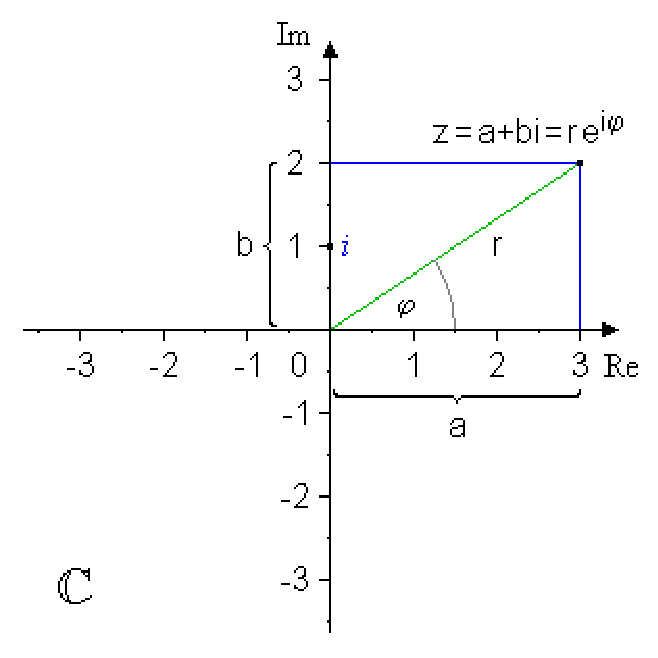
\epsfig{file=Abbildungen/gauss-ebene.eps, scale=0.7}
  \caption{Die Gau\3'sche Zahlen-Ebene.}
  \label{fig:gauss-ebene.eps}
\end{figure}

\vspace*{0.2cm}
\noindent
Bezeichnen wir den Betrag der komplexen Zahl $a + i \cdot b$ mit $r$, setzen wir also 
$r := |a + i \cdot b|$, so besteht zwischen dem in der Abbildung eingezeichneten Winkel $\varphi$
und den Komponenten $a$ und 
$b$ die Beziehung
\\[0.2cm]
\hspace*{1.3cm} $a = r \cdot \cos(\varphi)$ \quad und \quad $b = r \cdot \sin(\varphi)$.
\\[0.2cm]
Durch Division der zweiten Gleichung durch die erste Gleichung erhalten wir die Beziehung
\\[0.2cm]
\hspace*{1.3cm} $\tan(\varphi) = \bruch{b}{a}$.
\\[0.2cm]
Solange wir uns im ersten Quadranten der Ebene befinden, k\"{o}nnen wir daraus den Winkel $\varphi$ mit Hilfe
der Gleichung
\\[0.2cm]
\hspace*{1.3cm} $\varphi = \arctan\Bigl(\bruch{b}{a}\Bigr)$
\\[0.2cm]
ausrechnen.  Das Paar $\pair(r, \varphi)$ bezeichnen wir als die {\emph{\color{blue}Polarform}} der
komplexen Zahl $a + i \cdot b$, w\"{a}hrend wir das Paar $\pair(a,b)$ die {\emph{\color{blue}kartesische Darstellung}}
nennen.  Es ist instruktiv zu sehen, was passiert, wenn wir zwei
komplexe Zahlen in Polarform
\\[0.2cm]
\hspace*{1.3cm} 
$r_1 \cdot \cos(\varphi_1) + i \cdot r_1 \cdot \sin(\varphi_1)$ \quad und \quad
$r_2 \cdot \cos(\varphi_2) + i \cdot r_2 \cdot \sin(\varphi_2)$ 
\\[0.2cm]
multiplizieren.  Wir haben n\"{a}mlich
\\[0.2cm]
$
\begin{array}[t]{cl}
  & \bigl(r_1 \cdot \cos(\varphi_1) + i \cdot r_1 \cdot \sin(\varphi_1)\bigr) \cdot
    \bigl(r_2 \cdot \cos(\varphi_2) + i \cdot r_2 \cdot \sin(\varphi_2)\bigr)       \\[0.2cm]
= & r_1 \cdot r_2 \cdot
    \Bigl(\cos(\varphi_1) \cdot \cos(\varphi_2) - \sin(\varphi_1) \cdot \sin(\varphi_2) +
          i \cdot \bigl(\cos(\varphi_1) \cdot \sin(\varphi_2) + \sin(\varphi_1) \cdot \cos(\varphi_2)\bigr)
    \Bigr) \\[0.2cm]
= & r_1 \cdot r_2 \cdot
    \bigl(\cos(\varphi_1 + \varphi_2) + i \cdot \sin(\varphi_1 + \varphi_2) \bigr).
\end{array}
$
\\[0.2cm]
Im letzten Schritt dieser Umformung haben wir dabei die beiden 
\href{https://de.wikipedia.org/wiki/Formelsammlung_Trigonometrie#Additionstheoreme}{Additions-Theoreme}
\\[0.2cm]
\hspace*{1.3cm}
$\sin(\alpha + \beta) = \sin(\alpha) \cdot \cos(\beta) + \cos(\alpha) \cdot \sin(\beta)$ \quad und
\\[0.2cm]
\hspace*{1.3cm}
$\cos(\alpha + \beta) = \cos(\alpha) \cdot \cos(\beta) - \sin(\alpha) \cdot \sin(\beta)$
\\[0.2cm]
benutzt.   Wegen seiner Wichtigkeit halten wir das Ergebnis der obigen Rechnung in der folgenden Formel
fest:
\begin{equation}
  \label{eq:komplex_mult2}
  \bigl(\cos(\varphi_1) + i \cdot \sin(\varphi_1)\bigr) \cdot
  \bigl(\cos(\varphi_2) + i \cdot \sin(\varphi_2)\bigr)       
= \bigl(\cos(\varphi_1 + \varphi_2) + i \cdot \sin(\varphi_1 + \varphi_2) \bigr).
\end{equation}
Wir sehen, dass es einfach ist, komplexe Zahlen in der Polarform zu
multiplizieren: Die Winkel der Zahlen werden addiert.  Der \"{U}bersichtlichkeit halber habe ich
die Betr\"{a}ge $r_1$ und $r_2$ in der oberen Formel weggelassen.  

\subsection{Potenzen und allgemeine Wurzeln}
Ist eine komplexe Zahl in Polarform gegeben, so ist es leicht, die Zahl zu
potenzieren, denn aus Gleichung \ref{eq:komplex_mult2} folgt mit einem einfachen Induktions-Beweis,
dass f\"{u}r alle nat\"{u}rlichen Zahlen $n \in \mathbb{N}$ die Gleichung
\begin{equation}
  \label{eq:komplex_potenz}
  \bigl(\cos(\varphi) + i \cdot \sin(\varphi)\bigr)^n = \cos(n \cdot \varphi) + i \cdot \sin(n \cdot \varphi)
\end{equation}
gilt.  Diese Formel wird auch als \href{http://de.wikipedia.org/wiki/Abraham_de_Moivre}{\emph{Satz von de Moivre}} bezeichnet.  
Dieser Satz kann zum Ziehen beliebiger Wurzeln aus einer komplexen Zahl verwendet werden.  Um mit Hilfe dieses Satzes Wurzeln ziehen
zu k\"{o}nnen, bemerken wir zun\"{a}chst, dass die Funktionen $\sin(x)$ und $\cos(x)$ periodisch mit der Periode
$2 \cdot \pi$ sind, es gilt also
\\[0.2cm]
\hspace*{1.3cm}
$\sin(x + 2 \cdot \pi) = \sin(x)$ \quad und \quad
$\cos(x + 2 \cdot \pi) = \cos(x)$.
\\[0.2cm]
Diese Gleichungen lassen sich f\"{u}r beliebige $k \in \mathbb{N}$ zu
\\[0.2cm]
\hspace*{1.3cm}
$\sin(\varphi + 2 \cdot k \cdot \pi) = \sin(\varphi)$ \quad und \quad
$\cos(\varphi + 2 \cdot k \cdot \pi) = \cos(\varphi)$
\\[0.2cm]
verallgemeinern.  Wir \"{u}berlegen nun, f\"{u}r welche komplexe Zahlen der Form
\\[0.2cm]
\hspace*{1.3cm}
$z = \cos(\varphi) + i \cdot \sin(\varphi)$ \quad die Gleichung \quad $z^n = 1$
\\[0.2cm]
erf\"{u}llt ist.  Solche Zahlen bezeichnen wir als $n$-te Einheitswurzeln.  Da 
\\[0.2cm]
\hspace*{1.3cm}
$1 = \cos(2 \cdot k \cdot \pi) + i \cdot \sin(2 \cdot k \cdot \pi)$
\\[0.2cm]
gilt, muss nach Gleichung \ref{eq:komplex_potenz} f\"{u}r die Zahl $z = \cos(\varphi) + i \cdot \sin(\varphi)$
die Beziehung
\begin{equation}
  \label{eq:komplex_wurzel0}
\cos(2 \cdot k \cdot \pi) + i \cdot \sin(2 \cdot k \cdot \pi) =
\cos(n \cdot \varphi) + i \cdot \sin(n \cdot \varphi)  
\end{equation}
erf\"{u}llt sein, wenn $z^n = 1$ sein soll.  Die Gleichung \ref{eq:komplex_wurzel0} ist offensichtlich dann
erf\"{u}llt, wenn 
\\[0.2cm]
\hspace*{1.3cm}
$\varphi = \bruch{2 \cdot k \cdot \pi}{n}$
\\[0.2cm]
gilt, wobei wir $k$ auf die Elemente der Menge $\{0,1, \cdots, n-1\}$ beschr\"{a}nken k\"{o}nnen, denn gr\"{o}\3ere
Werte von $k$ liefern Winkel, die gr\"{o}\3er als $2 \cdot \pi$ sind.  Wir definieren daher
\\[0.2cm]
\hspace*{1.3cm}
\colorbox{red}{\framebox{\colorbox{blue}{\framebox{\colorbox{yellow}{
$\ds\zeta_n := \cos\Bigl(\frac{2 \cdot \pi}{n}\Bigr) + i \cdot \sin\Bigl(\frac{2 \cdot \pi}{n}\Bigr)$}}}}}
\\[0.2cm]
als die \emph{\color{blue}primitive} $n$-te Einheitswurzel und sehen, dass die Zahlen
\\[0.2cm]
\hspace*{1.3cm}
$\ds\zeta_n^k := \cos\Bigl(\frac{2 \cdot k \cdot \pi}{n}\Bigr) + i \cdot \sin\Bigl(\frac{2 \cdot k \cdot \pi}{n}\Bigr)$
\quad f\"{u}r $k \in \{ 0, 1, \cdots, n-1 \}$
\\[0.2cm]
dann alle $n$-ten Einheitswurzeln sind.

\example
F\"{u}r die primitive dritte Einheitswurzel $\zeta_3$ gilt
\\[0.2cm]
\hspace*{1.3cm}
$\ds\zeta_3 = \cos\Bigl(\frac{2 \cdot \pi}{3}\Bigr) + i \cdot \sin\Bigl(\frac{2 \cdot \pi}{3}\Bigr)
 = - \bruch{1}{2} + i \cdot \bruch{\sqrt{3\,}}{2}. 
$
\\[0.2cm] 
F\"{u}r $\zeta_3^2$ finden wir nach kurzer Rechnung
\\[0.2cm]
\hspace*{1.3cm}
$\ds\zeta_3^2 = \cos\Bigl(\frac{4 \cdot \pi}{3}\Bigr) + i \cdot \sin\Bigl(\frac{4 \cdot \pi}{3}\Bigr)
 = - \bruch{1}{2} - i \cdot \bruch{\sqrt{3\,}}{2}. 
$
\\[0.2cm]
Sie k\"{o}nnen leicht nachrechnen, dass sowohl $\zeta_3^3 = 1$ als auch $(\zeta_3^2)^3 = 1$ gilt.
\vspace*{0.2cm}

Mit Hilfe der $n$-ten Einheitswurzeln k\"{o}nnen wir jetzt allgemein f\"{u}r eine komplexe Zahl $z$ und eine
nat\"{u}rliche Zahl $n$ die L\"{o}sungen der Gleichung $r^n = z$ angeben.  Dazu ist zun\"{a}chst $z$ in
Polar-Koordinaten anzugeben.  Falls
\\[0.2cm]
\hspace*{1.3cm}
$z = r \cdot \bigl(\cos(\varphi) + i \cdot \sin(\varphi)\bigr)$
\\[0.2cm]
gilt, so ist offenbar f\"{u}r alle $k \in \{ 0, 1, \cdots, n - 1 \}$ die Zahl
\\[0.2cm]
\hspace*{1.3cm}
$\displaystyle s = \zeta_n^k \cdot \sqrt[n]{r\,} \cdot 
     \biggl(\cos\Bigl(\frac{\varphi}{n}\Bigr) + i \cdot \sin\Bigl(\frac{\varphi}{n}\Bigr) \biggr)
$
\\[0.2cm] 
eine L\"{o}sung der Gleichung $s^n = z$.

\example 
Wir berechnen alle L\"{o}sungen der Gleichung $r^3 = 1 + i$.  Dazu m\"{u}ssen wir zun\"{a}chst die Zahl
$1 + i$ in Polar-Koordinaten darstellen.  Setzen wir  
\\[0.2cm]
\hspace*{1.3cm} $\varphi = \arctan\Bigl(\bruch{1}{1}\Bigr) = \arctan(1) = \bruch{\pi}{4}$,
\\[0.2cm]
so gilt wegen $\sqrt{1^2 + 1^2\,} = \sqrt{2\,}$ offenbar
\\[0.2cm]
\hspace*{1.3cm} $\ds1 + i = \sqrt{2\,} \cdot \left(\cos\Bigl(\frac{\pi}{4}\Bigr) + i \cdot \sin\Bigl(\frac{\pi}{4}\Bigr)\right)$.
\\[0.2cm]
Damit erhalten wir dann als eine dritte Wurzel der Zahl $1 + i$ den Ausdruck
\\[0.2cm]
\hspace*{1.3cm}
$\ds r := \sqrt[6]{2\,} \cdot 
      \left(\cos\Bigl(\frac{\pi}{12}\Bigr) + i \cdot \sin\Bigl(\frac{\pi}{12}\Bigr)\right) 
$.
\\[0.2cm]
Ber\"{u}cksichtigen wir noch, dass die Werte der trigonometrischen Funktionen f\"{u}r das Argument
$\ds\frac{\pi}{12}$ bekannt sind, es gilt n\"{a}mlich
\\[0.2cm]
\hspace*{1.3cm} 
$\ds\cos\Bigl(\frac{\pi}{12}\Bigr) = \frac{1}{4} \cdot \bigl(\sqrt{6} + \sqrt{2}\bigr)$ \quad und \quad
$\ds\sin\Bigl(\frac{\pi}{12}\Bigr) = \frac{1}{4} \cdot \bigl(\sqrt{6} - \sqrt{2}\bigr)$,
\\[0.2cm]
so erhalten wir f\"{u}r $r$ den Ausdruck
\\[0.2cm]
\hspace*{1.3cm}
$r = \frac{1}{4} \cdot \sqrt[6]{2\,} \cdot
     \Bigl(\sqrt{6} + \sqrt{2} + i \cdot \bigl(\sqrt{6} - \sqrt{2}\bigr)\Bigr) 
$.
\\[0.2cm]
Ziehen wir hier $\sqrt{2}$ aus der Klammer und ber\"{u}cksichtigen, dass
\\[0.2cm]
\hspace*{1.3cm}
$\sqrt[6]{2} \cdot \sqrt{2} = 2^{\frac{1}{6}} \cdot 2^{\frac{1}{2}} =
 2^{\frac{4}{6}} =  2^{\frac{2}{3}} = \sqrt[3]{4}
$
\\[0.2cm]
gilt, so k\"{o}nnen wir $r$ als
\\[0.2cm]
\hspace*{1.3cm}
$r = \frac{1}{4} \cdot \sqrt[3]{4\,} \cdot \Bigl(\sqrt{3} + 1 + i \cdot \bigl(\sqrt{3} - 1\bigr)\Bigr)$
\\[0.2cm]
schreiben.  Die anderen beiden dritten Wurzeln erhalten wir daraus durch Multiplikation mit
$\zeta_3$ bzw.~$\zeta_3^2$.

\remark
Bei der obigen Rechnung hatten wir Gl\"{u}ck:  Erstens konnten wir f\"{u}r den Winkel $\varphi$ einen expliziten
Ausdruck, n\"{a}mlich $\frac{\pi}{4}$, angeben und zweitens konnten wir auch die Anwendung der trigonometrischen
Funktionen auf
\\[0.2cm]
\hspace*{1.3cm}
$\ds\frac{\varphi}{3} = \frac{\pi}{12}$ 
\\[0.2cm]
geschlossene Terme angeben.  Normalerweise
funktioniert das nicht und dann bleibt nur die numerische Rechnung. 

\exercise
Beweisen Sie, dass 
\\[0.2cm]
\hspace*{1.3cm}
$\ds\cos\Bigl(\frac{\pi}{12}\Bigr) = \frac{1}{4} \cdot \bigl(\sqrt{6} + \sqrt{2}\bigr)$ \quad und \quad
$\ds\sin\Bigl(\frac{\pi}{12}\Bigr) = \frac{1}{4} \cdot \bigl(\sqrt{6} - \sqrt{2}\bigr)$
\\[0.2cm]
gilt.  Verwenden Sie dazu den Satz von de Moivre, der im Skript als Gleichung
(\ref{eq:komplex_potenz}) angegeben ist. 
Au\3erdem d\"{u}rfen Sie in Ihrem Beweis die G\"{u}ltigkeit der Gleichungen
\\[0.2cm]
\hspace*{1.3cm}
$\ds\cos\Bigl(\frac{\pi}{6}\Bigr) = \frac{1}{2}\cdot\sqrt{3}$ \quad und \quad $\ds\sin\Bigl(\frac{\pi}{6}\Bigr) = \frac{1}{2}$
\\[0.2cm]
voraussetzen.
\exend

\section{Anwendung der komplexen Zahlen$^*$}
Wir k\"{o}nnen jetzt zwar mit komplexen Zahlen rechnen, wir haben aber bisher noch nicht gesehen, warum der 
Gebrauch von komplexen Zahlen \"{u}berhaupt notwendig ist.  Es gibt in der Mathematik eine Vielzahl von
Anwendung der komplexen Zahlen.  Stellvertretend m\"{o}chte ich an dieser Stelle die Fourier-Transformation
einer Funktion nennen, die in der Signalverarbeitung eine gro\3e Rolle spielt.  Darauf n\"{a}her einzugehen
ist aus Zeitgr\"{u}nden im Rahmen einer einf\"{u}hrenden Mathematik-Vorlesung leider unm\"{o}glich.  Auch f\"{u}r die
Anwendung komplexer Zahlen bei der L\"{o}sung von Differenzial-Gleichungen ist es jetzt noch zu fr\"{u}h.  Ich
m\"{o}chte statt dessen den historischen Weg gehen und zeigen, wie die komplexen Zahlen tats\"{a}chlich entdeckt
worden sind.  Ausgangspunkt unserer \"{U}berlegungen ist dabei die Gleichung
\\[0.2cm]
\hspace*{1.3cm}
$x^3 - 15 \cdot x - 4 = 0$.
\\[0.2cm]
Wir wollen alle m\"{o}glichen L\"{o}sungen dieser Gleichung bestimmen.  Um uns einen \"{u}berblick zu verschaffen,
skizzieren wir zun\"{a}chst die Funktion $x \mapsto x^3 - 15 \cdot x - 4$.  Wir erhalten den in Abbildung
\ref{fig:cubic.eps} auf Seite \pageref{fig:cubic.eps} gezeigten Graphen.

\begin{figure}[!ht]
  \centering
  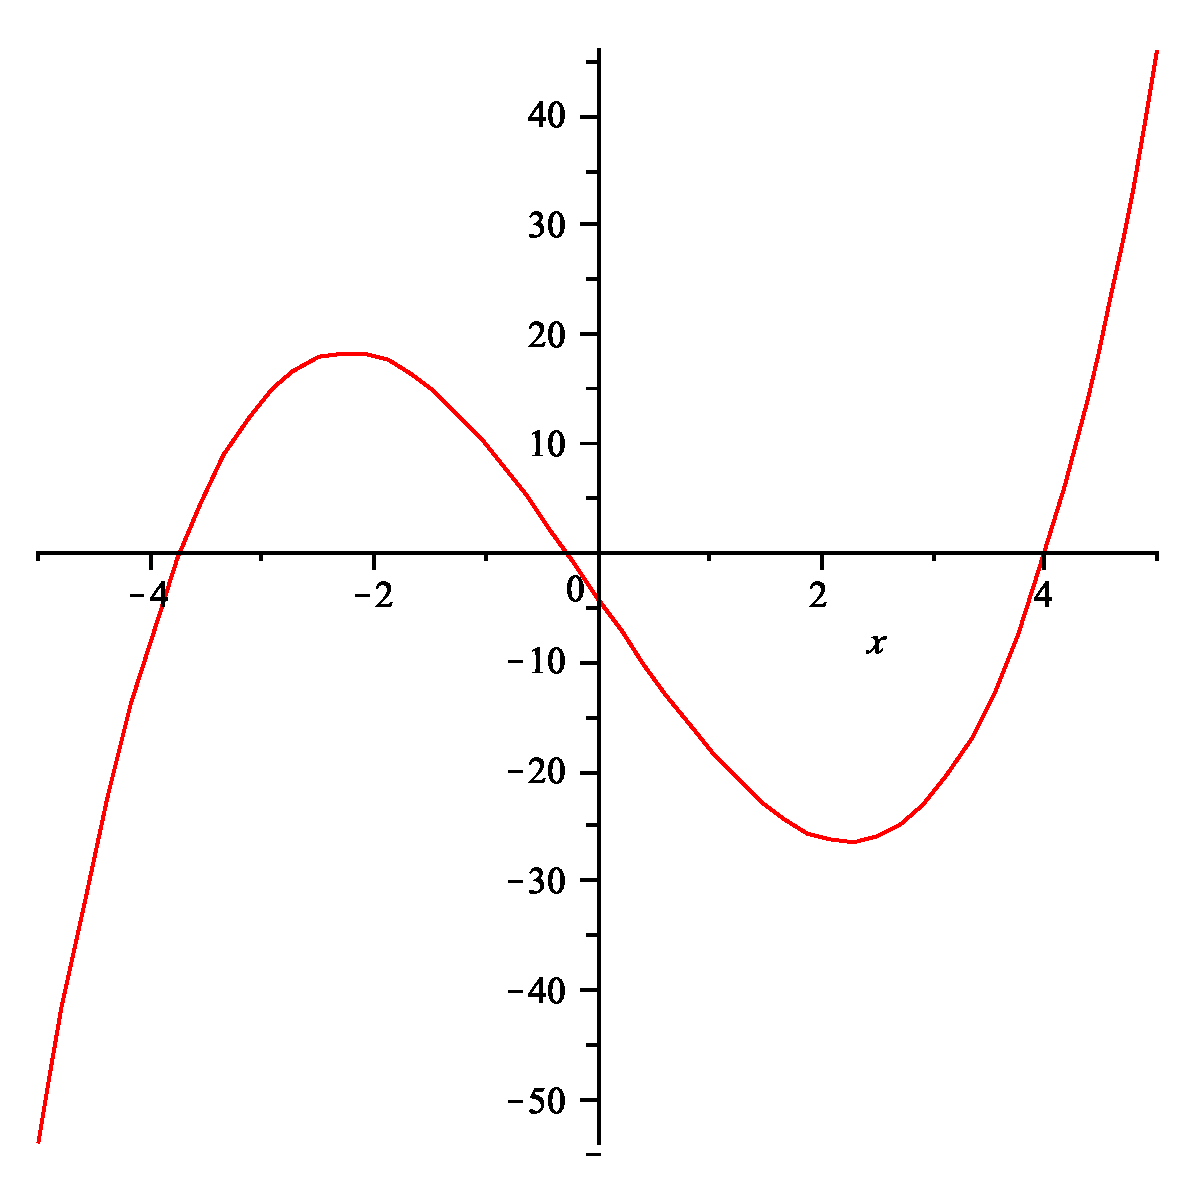
\epsfig{file=Abbildungen/cubic.eps, scale=0.4}
  \caption{Die Funktion $x \mapsto x^3 - 15 \cdot x - 4$.}
  \label{fig:cubic.eps}
\end{figure}

Es sieht so aus, als ob unsere Gleichung drei verschiedene L\"{o}sungen hat.  Um diese L\"{o}sungen zu bestimmen,
verallgemeinern wir unser Problem und versuchen, die kubische Gleichung
\begin{equation}
  \label{eq:cubic}
  x^3 - p \cdot x - q = 0  
\end{equation}
zu l\"{o}sen.  Wir machen dazu den Ansatz $x = u + v$.  Nun gilt
\\[0.2cm]
\hspace*{1.3cm}
$
\begin{array}[t]{lcl}
(u + v)^3 & = & (u + v)^2 \cdot (u + v)                                                           \\[0.2cm]
          & = & (u^2 + 2 \cdot u \cdot v + v^2) \cdot (u + v)                                     \\[0.2cm]
          & = & u^3 + u^2 \cdot v + 2 \cdot u^2 \cdot v + 2 \cdot u \cdot v^2 + u \cdot v^2 + v^3 \\[0.2cm]
          & = & u^3 + 3 \cdot u^2 \cdot v + 3 \cdot u \cdot v^2 + v^3                             \\[0.2cm]
          & = & 3 \cdot u \cdot v \cdot (u + v) + u^3 + v^3 
\end{array}
$
\\[0.2cm]
Daher k\"{o}nnen wir die kubische Gleichung mit dem Ansatz $x = u + v$ in die Gleichung
\\[0.2cm]
\hspace*{1.3cm}
$3 \cdot u \cdot v \cdot (u + v) + u^3 + v^3 - p \cdot (u + v) - q = 0$
\\[0.2cm]
\"{u}berf\"{u}hren, was wir noch zu
\\[0.2cm]
\hspace*{1.3cm}
$(3 \cdot u \cdot v - p) \cdot (u + v) + u^3 + v^3 - q = 0$
\\[0.2cm]
umschreiben.  Falls es uns gelingt, die Zahlen $u$ und $v$ so zu bestimmen, dass
\\[0.2cm]
\hspace*{1.3cm}
$p = 3 \cdot u \cdot v$ \quad und \quad $q = u^3 + v^3$
\\[0.2cm]
gilt, dann ist $x = u + v$ eine L\"{o}sung der kubischen Gleichung \ref{eq:cubic}.  Wir definieren
\\[0.2cm]
\hspace*{1.3cm}
$\alpha := u^3$ \quad und \quad $\beta := v^3$.
\\[0.2cm]
Damit lassen sich die Gleichungen f\"{u}r $u$ und $v$ umschreiben in
\\[0.2cm]
\hspace*{1.3cm}
$p^3 = 27 \cdot \alpha \cdot \beta$ \quad und \quad $q = \alpha + \beta$
\\[0.2cm]
Ist $\alpha \not= 0$, so folgt aus der ersten Gleichung
\\[0.2cm]
\hspace*{1.3cm}
$\beta = \bruch{p^3}{27 \cdot \alpha}$.
\\[0.2cm]
Setzen wir diesen Wert in die zweite Gleichung ein, so erhalten wir
\\[0.2cm]
\hspace*{1.3cm}
$q = \alpha + \bruch{p^3}{27 \cdot \alpha}$.
\\[0.2cm]
Multiplikation dieser Gleichung mit $\alpha$ liefert uns eine quadratische Gleichung f\"{u}r $\alpha$:
\\[0.2cm]
\hspace*{1.3cm}
$q \cdot \alpha = \alpha^2 + \bruch{p^3}{27}$.
\\[0.2cm]
Diese Gleichung stellen wir zu 
\\[0.2cm]
\hspace*{1.3cm}
$- \bruch{p^3}{27} = \alpha^2 - q \cdot \alpha$
\\[0.2cm]
um.  Addieren wir auf beiden Seiten die quadratische Erg\"{a}nzung $\ds\frac{q^2}{4}$, so erhalten wir
die quadratische Gleichung
\\[0.2cm]
\hspace*{1.3cm}
$\bruch{q^2}{4} - \bruch{p^3}{27} = \left(\alpha - \bruch{q}{2}\right)^2$.
\\[0.2cm]
Diese Gleichung hat offenbar die L\"{o}sung
\\[0.2cm]
\hspace*{1.3cm}
$\alpha = \bruch{q}{2} + \sqrt{\bruch{q^2}{4} - \bruch{p^3}{27}}$.
\\[0.2cm]
Wegen $q = \alpha + \beta$ folgt daraus f\"{u}r $\beta$
\\[0.2cm]
\hspace*{1.3cm}
$\beta = \bruch{q}{2} - \sqrt{\bruch{q^2}{4} - \bruch{p^3}{27}}$.
\\[0.2cm]
Wir pr\"{u}fen, ob f\"{u}r diese Werte von $\alpha$ und $\beta$ auch die zweite Bedingung 
\\[0.2cm]
\hspace*{1.3cm}
$\alpha \cdot \beta = \Bigl(\bruch{p}{3}\Bigr)^3$
\\[0.2cm]
erf\"{u}llt ist und finden tats\"{a}chlich
\\[0.2cm]
\hspace*{1.3cm}
$
\begin{array}[t]{lcl}
      \alpha \cdot \beta 
& = & \left(\bruch{q}{2} + \sqrt{\bruch{q^2}{4} - \bruch{p^3}{27}}\right) \cdot
      \left(\bruch{q}{2} - \sqrt{\bruch{q^2}{4} - \bruch{p^3}{27}}\right)        \\[0.2cm]
& = & \bruch{q^2}{4} - \left(\bruch{q^2}{4} - \bruch{p^3}{27}\right)             \\[0.2cm]
& = & \bruch{p^3}{27}.                                            
\end{array}
$
\\[0.2cm]
Ber\"{u}cksichtigen wir, dass $\alpha = u^3$, $\beta = v^3$ und $x = u + v$ ist,
so erhalten wir zur L\"{o}sung der kubischen Gleichung \ref{eq:cubic} die 
erstmals 1545 von \href{http://de.wikipedia.org/wiki/Gerolamo_Cardano}{Geralomo Cardano} ver\"{o}ffentlichte 
\emph{\color{blue}Cardanische Formel}
\\[0.2cm]
\hspace*{1.3cm}
\colorbox{red}{\framebox{\colorbox{blue}{\framebox{\colorbox{yellow}{
$x = \sqrt[3]{\bruch{q}{2} + \sqrt{\left(\bruch{q}{2}\right)^2 - \left(\bruch{p}{3}\right)^3\,}\;} +
     \sqrt[3]{\bruch{q}{2} - \sqrt{\left(\bruch{q}{2}\right)^2 - \left(\bruch{p}{3}\right)^3\,}\;}
$.}}}}}
\\[0.2cm]
In unserem urspr\"{u}nglichen Problem gilt $p = 15$ und $q = 4$.  Dann haben wir 
\\[0.2cm]
\hspace*{1.3cm}
$\alpha = \bruch{q}{2} + \sqrt{\left(\bruch{q}{2}\right)^2 - \left(\bruch{p}{3}\right)^3\,} =
 2 + \sqrt{4 - 125} = 2 + \sqrt{-121} = 2 + i \cdot 11
$.
\\[0.2cm]
Das ist aber eine komplexe Zahl, aus der wir jetzt noch die dritte Wurzel ziehen m\"{u}ssen.
An dieser Stelle haben wir Gl\"{u}ck, denn f\"{u}r die dritte Wurzel aus $2 + i \cdot 11$ und aus 
$2 - i \cdot 11$ l\"{a}sst sich jeweils ein expliziter Wert angeben, es gilt
\\[0.2cm]
\hspace*{1.3cm}
$u = \sqrt[3]{2 + i \cdot 11} = 2 + i$  \quad und \quad 
$v = \sqrt[3]{2 - i \cdot 11} = 2 - i$.
\\[0.2cm]
Wir wollen dieses Ergebnis im ersten Fall nachrechnen.  Es gilt
\\[0.2cm]
\hspace*{1.3cm}
$
\begin{array}[t]{lcl}
(2 + i)^3 & = & 2^3 + 3 \cdot 2^2 \cdot i + 3 \cdot 2 \cdot i^2 - i \\[0.2cm]
          & = & 8 - 6 + (12 - 1) \cdot i                            \\[0.2cm]
          & = & 2 + 11 \cdot i                            
\end{array}
$.
\\[0.2cm]
Damit finden wir als eine L\"{o}sung der kubischen Gleichung $x^3 - 15 \cdot x - 4 = 0$ den Wert
\\[0.2cm]
\hspace*{1.3cm}
$x_1 = 2 + 11 \cdot i + 2 - 11 \cdot i = 4$.
\\[0.2cm]
Sie sehen, dass wir ein Problem, dass mit komplexen Zahlen auf den ersten Blick nichts zu tun hat, durch die
Verwendung komplexer Zahlen l\"{o}sen konnten.
Der Vollst\"{a}ndigkeit halber wollen wir noch die anderen beiden L\"{o}sungen der kubischen Gleichung $x^3 - 15
\cdot x - 4 = 0$ bestimmen. 
Diese erhalten wir, wenn wir in der Cardanischen Formel auch die anderen M\"{o}glichkeiten f\"{u}r die dritte
Wurzel einsetzen.  Dabei m\"{u}ssen wir allerdings ber\"{u}cksichtigen, dass f\"{u}r die Zahlen $u$ und $v$ die
Nebenbedingung $3 \cdot u \cdot v = p$ gilt.  Multiplizieren wir beispielsweise $u$ mit $\zeta_3$ und 
$v$ mit $\zeta_3^2$, so haben wir
\\[0.2cm]
\hspace*{1.3cm}
$3 \cdot \zeta_3 \cdot u \cdot \zeta_3^2 \cdot v = 3 \cdot \zeta_3^3 \cdot u \cdot v = 3 \cdot u \cdot v = p$,
\\[0.2cm]
denn aus der Tatsache, dass $\zeta_3$ die dritte Einheitswurzel ist, folgt $\zeta_3^3 = 1$.  Als eine weitere L\"{o}sung erhalten wir dann
\\[0.2cm]
\hspace*{1.3cm}
$
\begin{array}[t]{lcl}
x_2 & = & \zeta_3 \cdot u + \zeta_3^2 \cdot v                               \\[0.2cm]
    & = & \zeta_3 \cdot (2 + i) + \zeta_3^2 \cdot (2 - i)                    \\[0.2cm]
    & = & \Bigl(- \bruch{1}{2} + i \cdot \bruch{\sqrt{3\,}}{2}\Bigr) \cdot (2 + i) + 
          \Bigl(- \bruch{1}{2} - i \cdot \bruch{\sqrt{3\,}}{2}\Bigr) \cdot (2 - i)   \\[0.3cm]
    & = & \bruch{1}{2} \cdot \bigl(-2 - \sqrt{3} + i \cdot (-1 + 2 \cdot \sqrt{3}) 
                                   -2 - \sqrt{3} + i \cdot ( 1 - 2 \cdot \sqrt{3})\bigr) \\[0.2cm]
    & = & - 2 - \sqrt{3}.  \\[0.2cm]
\end{array}
$
\\[0.2cm]
Auch hier ergibt sich also eine reelle L\"{o}sung.  F\"{u}r $x_3$ finden Sie nach einer \"{a}hnlichen Rechnung den Wert
\\[0.2cm]
\hspace*{1.3cm}
$x_3 = \zeta_3^2 \cdot u + \zeta_3 \cdot v = -2 + \sqrt{3}$.
\\[0.2cm]
Insgesamt zeigt dieses Beispiel, dass auch f\"{u}r Probleme, deren L\"{o}sungen reelle Zahlen sind, der Umweg
\"{u}ber die komplexen Zahlen sinnvoll sein kann.  Zum Abschluss m\"{o}chte ich noch bemerken, dass die
Verwendung komplexer Zahlen zur Bestimmung der Nullstellen eines Polynoms dritten Grades nicht
zwingend notwendig ist.  Die Nullstellen lassen sich auch auf trigonometrischem Wege bestimmen.  Dann ergibt
sich die Formel 
\\[0.2cm]
\hspace*{1.3cm}
\colorbox{red}{\framebox{\colorbox{blue}{\framebox{\colorbox{yellow}{
$\ds x_{k} = 2 \cdot \sqrt{\frac{p}{3}\;} \cdot 
    \cos\left(\frac{1}{3} \cdot \arccos\Bigl(\frac{3 \cdot q}{2 \cdot p} \cdot \sqrt{\frac{3}{p}}\Bigr)
    -(k-1) \cdot \frac{2 \cdot \pi}{3}\right)$ \quad for $k = 1,2,3$.}}}}}
\\[0.2cm]
Die trigonometrische Herleitung ist allerdings deutlich aufwendiger als die Herleitung die wir in diesem
Kapitel auf algebraischem Wege mit Hilfe der komplexen Zahlen gefunden haben.


\exercise
F\"{u}r welche $z \in \mathbb{C}$ gilt die Gleichung
\\[0.2cm]
\hspace*{1.3cm}
$\left(\bruch{1+z}{1-z}\right)^2 = -1$?
\exend
\pagebreak

\exercise
F\"{u}r welche Zahlen $x, y \in \mathbb{R}$ gilt
\\[0.2cm]
\hspace*{1.3cm}
$(5 + 6 \cdot i) \cdot (x - 3 \cdot i) = y - 3 \cdot i$?
\exend

\exercise
Welche komplexen Zahlen $z \in \mathbb{C}$ lassen sich in der Form
\\[0.2cm]
\hspace*{1.3cm}
$\bruch{1 + i \cdot x}{1 - i \cdot x} = z$ \quad mit $x \in \mathbb{R}$
\\[0.2cm]
schreiben? 
\vspace*{0.2cm}

\noindent
\textbf{Hinweis}:  Machen Sie f\"{u}r $z$ den Ansatz $z = a + b \cdot i$ mit $a,b \in \mathbb{R}$ und
setzen Sie diesen Ansatz in der obigen Gleichung f\"{u}r $z$ ein.  
\exend

\exercise
Bestimmen Sie mit Hilfe der Cardanischen Formel alle L\"{o}sungen der Gleichung 
\\[0.2cm]
\hspace*{1.3cm}
$x^3 = 3 \cdot x - 2$!
\exend


\section{Ausblick}
In diesem letzten Abschnitt stellen wir wichtige Formeln und Eigenschaften der komplexen Zahlen
zusammen, die wir allerdings erst im zweiten Semester beweisen k\"{o}nnen.

\subsection{Die Eulersche Formel}
Zwischen der Exponential-Funktion $x \mapsto e^x$ und den trigonometrischen Funktionen 
$x \mapsto \sin(x)$ und $x \mapsto \cos(x)$ gibt es einen wichtigen Zusammenhang, der als
{\href{https://de.wikipedia.org/wiki/Eulersche_Formel}{Eulersche Formel}} bekannt ist.  Es gilt
\\[0.2cm]
\hspace*{1.3cm}
\colorbox{red}{\framebox{\colorbox{blue}{\framebox{\colorbox{yellow}{
$e^{i \cdot \varphi} = \cos(\varphi) + i \cdot \sin(\varphi)$.}}}}}
\\[0.2cm]
Diese Formel k\"{o}nnen wir verstehen, wenn wir die
\href{https://de.wikipedia.org/wiki/Taylorreihe}{Reihenentwicklung} der beteiligten Funktionen
kennen.  In der Analysis werden wir sp\"{a}ter sehen, dass $e^x$, $\sin(x)$ und $\cos(x)$ wie folgt als Reihen
dargestellt werden k\"{o}nnen:
\begin{enumerate}
\item $\displaystyle e^x = 1 + x + \frac{1}{2} \cdot x^2 + \frac{1}{6} \cdot x^3 + \cdots = \sum\limits_{n=0}^\infty \frac{1}{n!} \cdot x^n$,
\item $\displaystyle \sin(x) = x - \frac{1}{6} \cdot x^3 + \cdots = \sum\limits_{n=0}^\infty \frac{(-1)^{n}}{(2 \cdot n + 1)!} \cdot x^{2 \cdot n + 1}$,
\item $\displaystyle \cos(x) = 1 -  \frac{1}{2} \cdot x^2 +  \frac{1}{24} \cdot x^4 + \cdots = \sum\limits_{n=0}^\infty  \frac{(-1)^{n}}{(2 \cdot n)!} \cdot x^{2 \cdot n}$.
\end{enumerate}
Setzen wir diese Reihen in der Eulerschen Formel ein und vergleichen die Koeffizienten von $x^n$, so
k\"{o}nnen wir die G\"{u}ltigkeit der Eulerschen Formel nachvollziehen.  Setzen wir in der Eulerschen Formel
f\"{u}r $\varphi$ den Wert $\pi$ ein, so erhalten wir die {\emph{\color{blue}Eulersche Identit\"{a}t}}
\\[0.2cm]
\hspace*{1.3cm}
\colorbox{red}{\framebox{\colorbox{blue}{\framebox{\colorbox{yellow}{
$e^{i \cdot \pi} = -1$.}}}}}
\\[0.2cm]
Diese Formel zeigt, dass zwischen der \href{https://de.wikipedia.org/wiki/Kreiszahl}{Kreiszahl} $\pi$ und der 
\href{https://de.wikipedia.org/wiki/Eulersche_Zahl}{Eulerschen Zahl} $e$ ein Zusammenhang besteht,
der durch die komplexen Zahlen hergestellt wird.


\subsection{Der Fundamentalsatz der Algebra}
In diesem Abschnitt zitieren wir (ohne Beweis) den sogenannten \emph{\color{blue}Fundamentalsatz der Algebra}.  Dieser Satz
besagt, dass jedes nicht-konstante Polynom  
\\[0.2cm]
\hspace*{1.3cm}
$p(z) = \sum\limits_{i=0}^n a_i \cdot z^i$ \quad mit $n \geq 1$ und $a_n \not=0$
\\[0.2cm]
im K\"{o}rper der komplexen Zahlen eine Nullstelle hat, d.h.~es gibt ein $z_1 \in \mathbb{C}$, so dass
$p(z_1) = 0$ ist.  Mit Hilfe der Polynom-Division k\"{o}nnen wir die Nullstelle $z_1$ aus dem Polynom $p(z)$
heraus dividieren und $p(z)$ in der Form
\\[0.2cm]
\hspace*{1.3cm}
$p(z) = (z - z_1) \cdot p_1(z)$
\\[0.2cm]
schreiben, wobei $p_1(z)$ dann ein Polynom vom Grad $n-1$ ist.  Falls $n-1 \geq 1$ ist, hat auch
$p_1(z)$ eine Nullstelle $z_2$, die wir aus $p_1(z)$ heraus dividieren k\"{o}nnen, so dass wir $p_1(z)$
in der Form
\\[0.2cm]
\hspace*{1.3cm}
$p_1(z) = (z- z_2) \cdot p_2(z)$
\\[0.2cm]
schreiben k\"{o}nnen, wobei $p_2(z)$ ein Polynom vom Grad $n-2$ ist.  Durch Iteration dieses Verfahrens
finden wir also insgesamt $n$ Zahlen $z_1, z_2, \cdots, z_n$, so dass wir $p(z)$ als das Produkt
\\[0.2cm]
\hspace*{1.3cm}
$p(z) = (z-z_1) \cdot (z-z_2) \cdot \mbox{\dots} \cdot (z-z_{n-1}) \cdot (z - z_n)$
\\[0.2cm]
schreiben k\"{o}nnen.  Dabei brauchen die komplexen Zahlen $z_i$ keineswegs paarweise verschieden zu sein,
sondern sie k\"{o}nnen auch durchaus gleich sein.  Wir bemerken noch, dass diese Darstellung bis auf die
Reihenfolge der $z_i$ eindeutig sein muss, denn die $z_i$ sind genau die Nullstellen des Polynoms
$p(z)$ und ein Polynom vom Grade $n$ hat, wie die obigen \"{U}berlegungen zeigen, h\"{o}chstens $n$
verschiedene Nullstellen.
\vspace*{0.2cm} 

\noindent
\textbf{Bemerkung}: Der Fundamentalsatz der Algebra zeigt, dass die Struktur der komplexen Zahlen
aus algebraischer Sicht wesentlich reichhaltiger als die Struktur der reellen Zahlen ist, denn in
den komplexen Zahlen hat jede Gleichung der Form
\\[0.2cm]
\hspace*{1.3cm}
$z^n + a_{n-1} \cdot z^{n-1} + \cdots + a_1 \cdot z + a_0 = 0$ \quad f\"{u}r $n \geq 1$
\\[0.2cm]
eine L\"{o}sung.  Es ist also nicht nur so, dass wir die Gleichung
\\[0.2cm]
\hspace*{1.3cm}
$z^2 + 1 = 0$
\\[0.2cm]
in den komplexen Zahlen l\"{o}sen k\"{o}nnen, sondern in den komplexen Zahlen k\"{o}nnen wir tats\"{a}chlich
j\underline{ede} quadratische Gleichung l\"{o}sen.  Dar\"{u}ber hinaus k\"{o}nnen wir auch jede kubische
Gleichung l\"{o}sen und ganz allgemein hat jede Gleichung $n$-ten Grades eine L\"{o}sung, solange $n$ nur
positiv ist.  Dies ist einer von vielen Gr\"{u}nden, warum die komplexen Zahlen so wichtig sind.
\vspace*{0.2cm}

\noindent
Der Beweis des Fundamentalsatzes der Algebra ben\"{o}tigt Hilfsmittel aus der Analysis, die wir nicht
zur Verf\"{u}gung haben.  Der Beweis ist auch nicht ganz einfach: Das k\"{o}nnen Sie beispielsweise der
Tatsache entnehmen, dass der bedeutendste Mathematiker, der je gelebt hat, 
\href{http://de.wikipedia.org/wiki/Carl_Friedrich_Gauss}{Carl Friedrich Gau\3}
diesen Satz 1799 in seiner Dissertation bewiesen hat.  Der Beweis, den Gau\3 damals gab, enthielt
allerdings noch eine L\"{u}cke.  Der erste vollst\"{a}ndige Beweis des Fundamentalsatzes der Algebra wurde 
1806 von \href{http://en.wikipedia.org/wiki/Jean-Robert_Argand}{Jean-Robert Argand} angegeben.

%%% Local Variables:  
%%% mode: latex
%%% TeX-master: "lineare-algebra"
%%% End: 
